\section{Data}
\label{sec:data}

Luminous red galaxies (LRGs) are massive galaxies that populate massive halos, lack active star formation, and are highly biased tracers of dark matter gravitational field. A distinct break around 4000 \AA~in the LRG spectrum is often utilized to determine their redshifts accurately. LRGs are widely targeted in previous galaxy redshift surveys \citep[see, e.g.,][]{eisenstein2001spectroscopic, prakash2016sdss}, and their clustering and redshift properties are well studied \citep[see, e.g.,][]{ross2020MNRAS.498.2354R, gilmarin2020MNRAS.498.2492G, bautista2021MNRAS.500..736B, chapman2022MNRAS.516..617C}. 

DESI is designed to collect spectra of millions of LRGs covering the redshift range $0.2<z<1.35$. DESI spectroscopy selects its targets from the DESI Legacy Imaging Surveys. The Legacy Surveys consists of three ground-based surveys that provide photometry of the sky in the optical $g$, $r$, and $z$ bands between 2014 and 2019. These surveys include the Mayall $z$-band Legacy Survey using the Mayall telescope at Kitt Peak \citep[MzLS;][]{dey2018overview}, the Beijing–Arizona Sky Survey using the Bok telescope at Kitt Peak \citep[BASS;][]{zou2017project}, and the Dark Energy Camera Legacy Survey on the Blanco 4m telescope \citep[DECaLS][]{flaugher2015dark}. As shown in Figure \ref{fig:ng}, the BASS and MzLS surveys observed the same footprint in the North Galactic Cap (NGC) while the DECaLS program observed both caps around the galactic plane; the BASS+MzLS footprint is separated from the DECaLS NGC at DEC $> 32.375$ degrees, although there is an overlap between the two regions for calibration purposes \citep{dey2018overview}. Additionally, the DECaLS program integrates observations executed from the Blanco instrument under the Dark Energy Survey \citep{abbott2016dark}, which cover about $1130 \deg^{2}$ of the South Galactic Cap (SGC) footprint. The DESI imaging catalogs also integrate the $3.4$ (W1) and $4.6$ $\mu m$ (W2) infrared photometry from the Wide-Field Infrared Explorer \citep[WISE;][]{wise2010AJ....140.1868W, meisner2018RNAAS...2....1M}.  \bbk{[Would it be worth including a map of what survey has covered what footprint?]}\mr{MR: I annotated Fig. 2, what do you think?}\bbk{Looks great, thank you}

\subsection{DESI imaging LRGs}
Our sample of LRGs is drawn from the DESI Legacy Imaging Surveys Data Release 9 \citep[DR9;][]{dey2018overview} using the color-magnitude selection criteria designed for the \mr{DESI 1\% survey}, described as the SV3 selection in more detail in \cite{zhou2022target}. The color-magnitude selection cuts are defined in the $g$, $r$, $z$ bands in the optical and $W1$ band in the infrared, as summarized in Table \ref{tab:ts}. The selection cuts are developed differently for each imaging survey to reach an almost uniform target surface density despite different survey efficiency and photometric calibration between DECaLS and BASS+MzLS. The implementation of these selection cuts in the DESI data processing pipeline is explained in \cite{myers2022}. The redshift distribution of our galaxy sample is inferred from DESI spectroscopy during the Survey Validation phase. A constant clustering amplitude is assumed for linear bias which is supported by data \citep{zhou2021clustering}. Figure \ref{fig:nz} shows the redshift distribution (solid black line) and the evolution of linear bias (dashed red line) for our sample of LRGs.

\begin{figure}
 \centering
 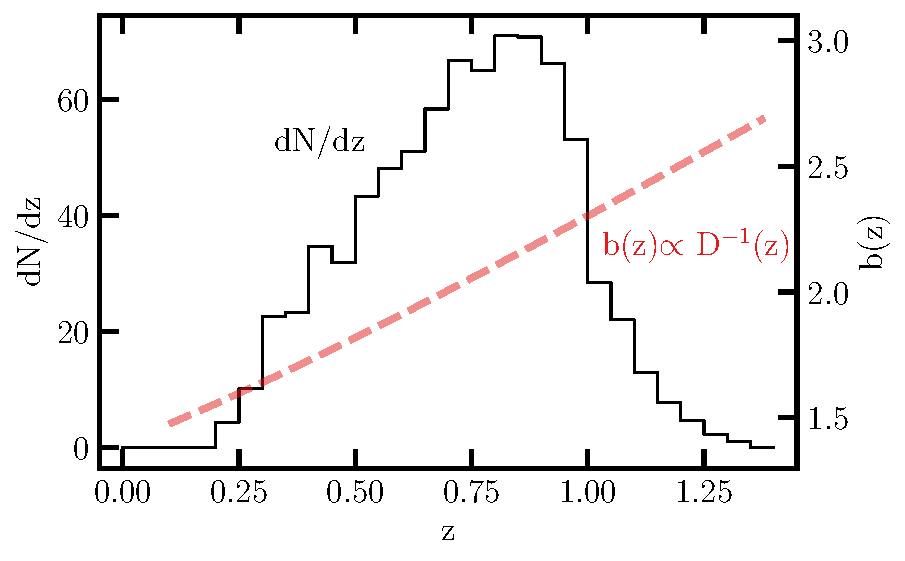
\includegraphics[width=0.45\textwidth]{figures/nz_lrg.pdf}
 \caption{The redshift distribution (solid line) and bias evolution (dashed line) of DESI LRG targets. The redshift distribution is determined by DESI spectroscopy, and a constant clustering amplitude is assumed for linear bias.}
 \label{fig:nz}
\end{figure}

\begin{table*}
\caption{Selection criteria for the DESI-like LRG targets \citep{zhou2022target}. Magnitudes are corrected for MW extinction. $z_{\rm fiber}$ represents the z-band fiber magnitude which corresponds to the expected flux within a DESI fiber.} \label{tab:ts}
 \centerline{%
 \begin{tabular}{lll}
 \hline
 \hline
 \textbf{Footprint} & \textbf{Criterion} &\textbf{Description}\\
 \hline
 \hline  
 & $z_{\rm fiber} < 21.7$ & Faint limit \\
  DECaLS & $z - W1 > 0.8 \times (r - z) - 0.6$ & Stellar rejection \\
 & $[(g-r >1.3)~{\rm AND}~((g-r) > -1.55*(r-W1) + 3.13)]~{\rm OR}~(r -W 1 > 1.8)$ & Remove low-z galaxies \\
 & $[(r-W1 > (W1 - 17.26)*1.8)~{\rm AND}~(r - W1 > W1 - 16.36)]~{\rm OR}~(r-W1 > 3.29)$ & Luminosity cut \\ 
 \hline
 & $z_{\rm fiber} < 21.71$ & Faint limit \\
 BASS+MzLS & $z - W1 > 0.8 \times (r - z) - 0.6$ & Stellar rejection \\
 & $[(g-r >1.34)~{\rm AND}~((g-r) > -1.55*(r-W1) + 3.23)]~{\rm OR}~(r -W 1 > 1.8)$ & Remove low-z galaxies \\
 & $[(r-W1 > (W1 - 17.24)*1.83)~{\rm AND}~(r - W1 > W1 - 16.33)]~{\rm OR}~(r-W1 > 3.39)$ & Luminosity cut \\ 
 \hline
 \end{tabular}}
\end{table*}

\begin{figure*}
 \centering
 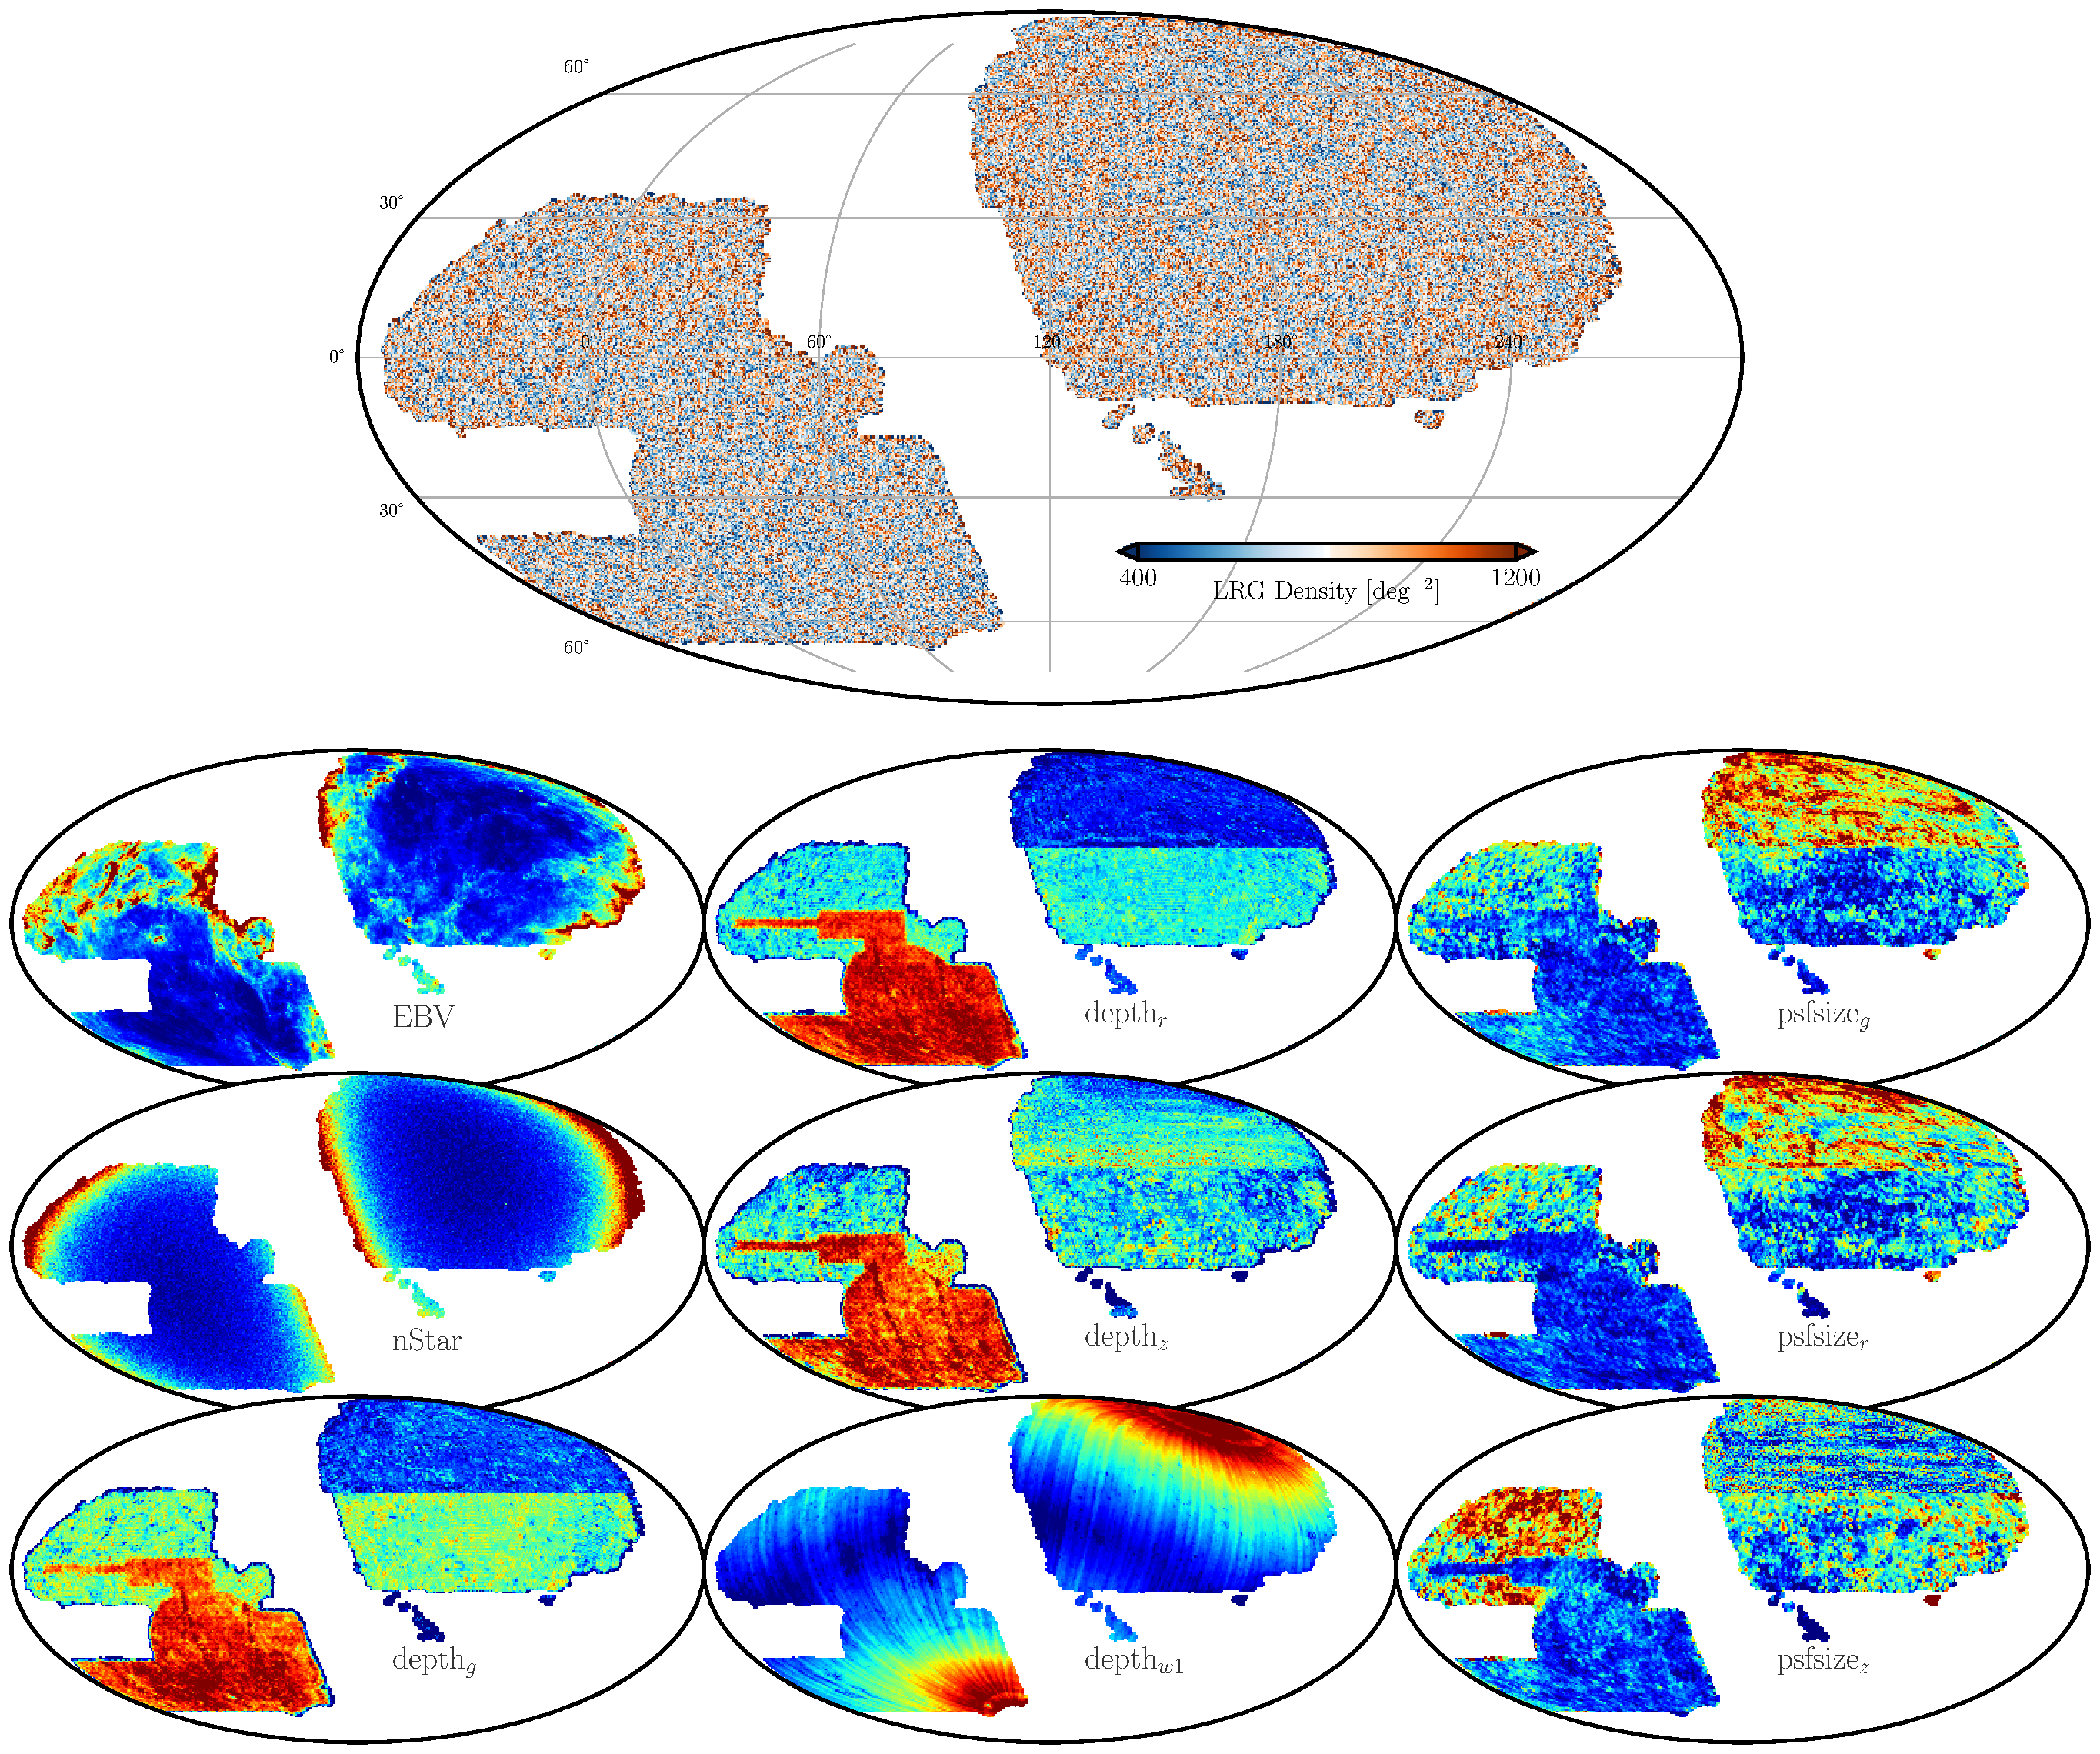
\includegraphics[width=0.99\textwidth]{figures/dr9data.pdf}
 \caption{Top: The DESI LRG target density map before imaging systematics correction in Mollweide projection. Spurious disconnected islands from the North footprint and declination below $-30$ from the South footprint are removed for the analysis due to potential calibration issues (see text). Bottom: Mollweide projections of the DESI DR9 imaging properties (survey depth and astronomical seeing/psfsize) and MW foregrounds (extinction and local stellar density) in celestial coordinates. Two external imaging systematic maps are neutral hydrogen column density and photometric calibration maps (not shown), which only used for robustness tests. The imaging values are color coded to increase from blue to red.}
 \label{fig:ng}
\end{figure*}

The LRG sample is masked rigorously for foreground bright stars, bright galaxies, and clusters of galaxies\footnote{See \url{https://www.legacysurvey.org/dr9/bitmasks/} for maskbit definitions.} to further reduce stellar contamination \citep{zhou2022target}. Then, the sample is binned into \textsc{HEALPix} \citep{gorski2005healpix} pixels at $\textsc{nside}=256$ to construct the 2D density map with an average surface density of $800$ galaxies per square degree covering around $14000$ square degrees (as shown in Figure \ref{fig:ng}). The LRG density is corrected for the pixel incompleteness and lost areas using a catalog of random points, hereafter referred to as randoms, uniformly scattered over the footprint with the same cuts and masks applied. The LRG density map exhibits some large-scale spurious fluctuations, even though that DESI-like LRGs are selected brighter than the imaging survey depth limits. Specifically, the SGC footprint exhibits some systematic under-density while there is some systematic over-density near the survey boundaries in the NGC.

\subsubsection{Imaging properties}
In this paper, various imaging properties, which can be considered as potential sources of systematic error, are mapped into \textsc{HEALPix} of \textsc{nside}$=256$ (Figure \ref{fig:ng}). The maps include local stellar density constructed from point-like sources with a G-band magnitude in the range $12 \leq G < 17$ from the Gaia DR2 \citep[see,][]{gaiadr2, myers2022}; Galactic extinction E[B-V] from \cite{schlegel1998maps}; survey depth (galaxy depth in $g$, $r$, and $z$ and PSF depth in W1) and astronomical seeing (psfsize) in $g$, $r$, and $z$. These maps have been previously identified as potential sources of imaging systematics in DESI-like LRGs \cite{zhou2022target}. We also consider two external maps for the neutral hydrogen column density (HI) from \cite{2016A&A...594A.116H} and photometric calibration in the z-band (CALIBZ) from \mr{CITE} for robustness tests.

Each imaging map carries its characteristic fluctuations, which correlate with the LRG density map. For instance, large-scale fluctuations can be associated with stellar density, extinction, or survey depth; while small scale-fluctuations can be related to psfsize variations. Upon visual inspection, the under-dense regions of LRGs in the SGC can be associated with varying survey depth, while the over-dense regions in the NGC can be connected to galactic dust or extinction. Some regions of the DR9 footprint are removed from our analysis to avoid potential photometric calibration issues. Some of these regions are disconnected from the main footprint (e.g., spurious islands in the NGC) or different types of standard starts were used for their calibration (DEC$<-30$ in the SGC). The potential impact of these declination cuts on our $\fnl$ constraints is explored in Section \ref{sec:results}. 

\begin{figure}
\centering
 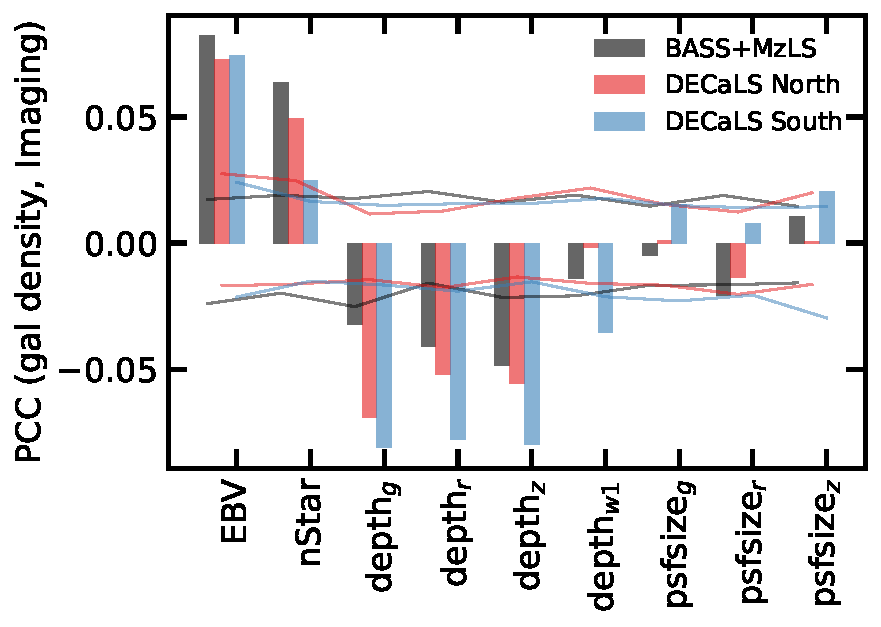
\includegraphics[width=0.45\textwidth]{figures/pcc.pdf} 
 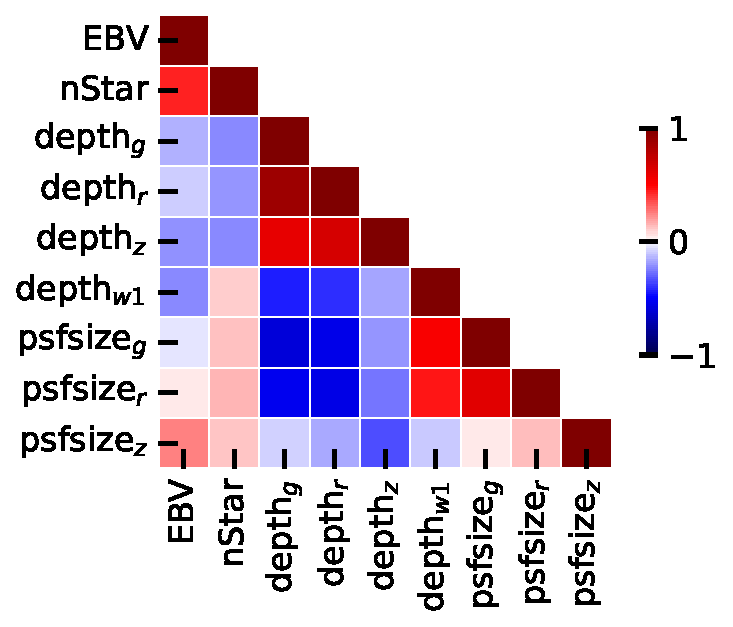
\includegraphics[width=0.45\textwidth]{figures/pccx.pdf}  
 \caption{Top: The Pearson correlation coefficient between the DESI LRG target density and imaging properties in BASS+MzLS, DECaLS North, and DECaLS South. Solid horizontal curves represent the $95\%$ confidence regions estimated from 100 simulated lognormal density maps. Bottom: The Pearson correlation matrix of imaging properties for the DESI footprint.}
 \label{fig:pcc}
\end{figure}

Figure \ref{fig:pcc} shows the Pearson correlation coefficient between the DESI LRG target density and the imaging systematics maps for the three imaging regions (DECaLS North, DECaLS South, and BASS+MzLS) in the top panel. The horizontal curves represent the $95\%$ confidence regions, and are constructed by cross correlating 100 synthetic lognormal density fields and the imaging systematic maps. Figure \ref{fig:pcc} (bottom) shows the correlation matrix among the imaging systematics maps for the DESI footprint. There is \mr{statistically significant} correlations between the LRG density and depth, extinction, and stellar density. There is \mr{no significant} correlations between the LRG density and the $W1$-band depth and psfsize. Significant inner correlations exist among the imaging systematic maps themselves, especially between the local stellar density and Galactic extinction; also, the $r$-band and $g$-band survey properties are more correlated with each other than with the $z$-band. \mr{The Spearman-r correlation coefficient is also applied to measure the relationship between the DESI target density and imaging systematic maps, but no significant differences between the Spearman and Pearson results are found.} 


\subsubsection{Imaging weights}
The effects of observational systematics in the DESI targets have been studied in great detail \cite[see, e.g.,][]{kitanidis2020imaging, zhou2021clustering, chaussidon2022angular}. There are several approaches for handling imaging systematic errors, broadly classified into data-driven backward modeling and simulation-based forward modeling. The general idea behind these approaches is to use the available data or simulations to learn or forward model the relationship between the observed target density and the imaging systematic maps, and to use this relationship, which is often described by a set of \textit{imaging weights}, to correct for systematic errors. \bbk{\sout{An}}other techniques for mitigating the effect of imaging systematics rel\bbk{y} on cross-correlating different tracers of dark matter to reduce excess clustering signals, as each tracer might respond differently to a source of systematic error \citep[see, e.g.,][]{giannantonio2014improved}. These methods have their limitations and strengths \citep[see, e.g.,][for a review]{2021MNRAS.503.5061W}.

In this paper, a backward modeling approach is applied to the data. Both linear multivariate and nonlinear neural network regressions are used to correct for imaging systematics. One potential problem that can arise in the mitigation process is \textit{over-correction}, which occurs when the corrections applied to the data are too strong, leading to the removal of the clustering signal and the introduction of additional biases in the inferred parameter. These effects are demonstrated to be negligible for observables like BAO and RSD \citep{merz2021clustering}; however, they can significantly impact the clustering power on large scale, and thus induce biases in $\fnl$ constraints \citep{mueller2022primordial, rezaie2021primordial}. The other problem is that the imaging systematic maps are strongly correlated (Figure \ref{fig:pcc}). It is crucial to develop techniques to control over-correction and to reduce dimensionality of the problem, in the hope of ensuring that the constraints are as accurate and reliable as possible, in particular for problems such as local primordial non-Gaussianity and other features in the primordial power spectrum \citep{beutler2019primordial}. Using more maps increases the input noise and the likelihood of overcorrection. With the objective of minimizing the cross-correlations between the LRG target density (after correction) and the imaging systematic maps, our plan is to obtain various levels of corrections ranging from conservative to extreme by using the following combinations:
\begin{enumerate}[itemindent=*]
\item \textbf{Conservative I}: Extinction, depth in z.
\item \textbf{Conservative II}: Extinction, depth in z, psfsize in r.
\item \textbf{All Maps}: Extinction, depth in $grzW1$, psfsize in $grz$.
\end{enumerate}
In addition to these sets of imaging systematic maps, we also explore including three extra maps for local stellar density (nStar), magnitude calibration in the z band (CALIBZ), and neural hydrogen column density (HI). 

Both linear and neural network models are trained on each imaging region separately since the Pearson correlation coefficient analysis indicated that each imaging region responds differently to each imaging map (Figure \ref{fig:pcc}). The optimal parameters associated with the linear and neural networks models are found by optimizing the negative Poisson log-likelihood, $\lambda - \rho \log(\lambda)$, measured between the observed target density $\rho$ and the model output for the predicted density $\lambda$ given only imaging properties \textbf{x} as input. No spatial coordinates are included in input \textbf{x} to avoid over-correction. The expected mean number of galaxies is defined as $\lambda(\textbf{x}) \equiv \log (1+e^{f(\textbf{x})})$, where either linear multivariate regression or nonlinear artificial neural networks is used to estimate $f$. 

The linear multivariate model only uses the imaging systematic maps up to the linear power. The observed target density $\rho$ is related to the imaging properties $\textbf{x}$ for pixel $i$ by,
\begin{equation}
    \rho_{i} = a_{0} + \sum_{j} a_{j}x_{ji},
\end{equation}
where $x_{ji}$ is the value for the $j^{\rm th}$ imaging map in pixel $i$ and $a_{j}$ is the corresponding parameter, yet to be found by optimization with a random search method called Monte Carlo Markov Chain (MCMC) using the implementation of \textsc{emcee} \citep{2013PASP..125..306F}. As our data size dominates the number of parameters for the linear model, no training-validation split is performed on the linear model. Our neural network-based mitigation approach uses the implementation from \cite{rezaie2021primordial}; which trains an ensemble of 20 neural network models on the data. Each neural network is a fully-connected feed forward architecture that starts with the imaging values as input in the first layer, three hidden layers with 20 rectifier activation function units, and a single identity function unit in the output layer. The rectifier activation function is defined as ${\rm max}(0, x)$. This simple form of nonlinearity is very effective in enabling deep neural networks to learn complex functions \citep{nair2010rectified}. Unlike linear regression, neural networks are prone to fitting noise, i.e., excellent performance on training data and poor performance on unseen data. Therefore, our analysis uses a training-validation-testing split to ensure that the network is well-optimized and generalizes well to unseen data. Specifically, $60\%$ of the LRG data is used for training, $20\%$ is used for validation, and $20\%$ is used for testing. The neural network models are tested on the entirety of the LRG sample with the technique of permuting the choice of the training, validation, or testing sets \citep{arlot2010survey}. The neural networks are trained for up to 70 training epochs with the gradient descent \textsc{Adam} optimizer \citep{2017arXiv171105101L}. With this approach, the neural network parameters are updated iteratively following the gradient of the negative Poisson log-likelihood. The step size of the parameter updates is controlled via the learning rate hyper-parameter, which is initialized with a grid search and is set to dynamically vary between two boundary values of $0.001$ and $0.1$ to avoid local minima \citep{2016arXiv160803983L}. At each training epoch, the neural network models are applied to the validation set, and ultimately the models with the best performance are saved as the best models and applied to the test set. With cross-validation technique, the model predictions from the different test sets are aggregated together to form the predicted target density map into \textsc{HEALPix} of \textsc{nside} $=256$. The imaging weights are then defined as the inverse of the normalized predicted target density, and applied to the target density to correct for imaging systematics.

A visual inspection of the predicted target density maps reveals that most of the large-scale spurious fluctuations are explained by just extinction and depth in the z-band. Adding psfsize in the r-band results in more small-scale spurious fluctuations in the predicted target density maps. Our inspection shows that using all of the imaging systematic maps as input for regression does not provide more information, which is expected from highly correlated predictors (Figure \ref{fig:pcc}). Given the same set of inputs, the neural network-based weights show more small-scale spurious fluctuations which can be associated with the higher flexibility of the underlying model. Both approaches yield large-scale spurious fluctuations consistent with the LRG target density; for instance, both models predict a higher density of LRGs near the boundaries where the DESI imaging surveys observed regions of high extinction or high stellar density near the galactic plane. These over-dense regions are likely contaminated artifacts entering the LRG selection, e.g., stellar contaminants or other artifacts because of obscured photometry from extinction. This is interesting since the target selection cuts use extinction corrected magnitudes. Further robustness tests on these weights are discussed in Section \ref{sec:method}, and their impacts on $\fnl$ are presented in Section \ref{sec:results}.


\subsection{Synthetic lognormal density fields}\label{ssec:mocks}
Density fluctuations of galaxies on large scales can be approximated with lognormal distributions \citep{coles1991}. Unlike N-body simulations, simulating lognormal density fields is not computationally intensive, and allows quick and robust validation of data analysis pipelines. These mocks are therefore considered useful for our study since the signature of local PNG appears on large-scales and small scale clustering is not used. The package \textsc{FLASK} \citep[Full-sky Lognormal Astro-fields Simulation Kit;][]{Xavier_2016} is employed to generate ensembles of synthetic lognormal density maps that mimic the redshift and angular distributions of the DR9 LRG targets. Two universes with $\fnl=0$ and $76.92$ are considered. For each $\fnl$, 1000 realizations are generated assuming a redshift dependent bias $b(z)=1.43/D(z)$ \citep[see, e.g.,][]{zhou2021clustering}. The analysis adapts a fiducial cosmology from a flat $\Lambda$CDM universe, including one massive neutrino with $m_{\nu}=0.06$ eV, while the rest of cosmological parameters is deducted from Planck 2018 \citep{aghanim2020planck},
\begin{equation*}
 h = 0.67, \Omega_{M}=0.31, \sigma_{8}=0.8, {\rm and}~ n_{s}=0.97.
\end{equation*}
The same fiducial cosmology is used throughout this paper unless specified otherwise. The robustness of our constraints against the fiducial cosmology is explored in Section \ref{sec:results}.

\subsubsection{Contaminated mocks}
The linear multivariate model is trained with extinction, depth in z, and psfsize in r (\textit{conservative II}), and is applied to introduce synthetic spurious fluctuations in the lognormal density fields. The motivation for choosing a linear model for the contamination is to assess how much of the clustering signal can be removed by applying more flexible and rigorous models (based on neural networks) for correcting the effect of imaging systematics. The parameters of the linear model are fit on the DESI LRG target sample, separately on each imaging survey. The contamination model for each simulation is uniquely and randomly drawn from the parameter space constraint by MCMC. The same contamination model is used for both the $\fnl=0$ and $76.92$ simulations.

Similar to the analysis for the DESI LRG targets, the linear and neural network methods are applied to each simulation, with and without PNG or with and without systematics, to derive the imaging weights. No prior knowledge is used regarding the underlying model or the input imaging systematic maps for contamination, to simulate a realistic scenario. Section \ref{sec:method} presents how the simulation results are incorporated to calibrate $\fnl$ biases due to over-correction. 